\documentclass[10pt,a4paper]{book}
\usepackage[utf8]{inputenc}
\usepackage[french]{babel}
\usepackage[T1]{fontenc}
\usepackage{amsmath}
\usepackage{amsfonts}
\usepackage{amssymb}
\usepackage{graphicx}
\author{ Antoine Robin}
\title{Warhammer - campagne}
\newcommand{\nomadversaire}{culte inconnu}
\begin{document}
\maketitle
\tableofcontents
\chapter{Arcs narratifs}
\section{Arc principal : l'influence du chaos}
Au cours de cette campagne, les PJs vont affronter l'influence pernicieuse, mais subtile d'un culte du chaos, jusqu'au déclenchement de ses plans machiavéliques.
\subsection{Synopsis}
 C'est un arc narratif en trois actes : lors du premier, les actes du culte seront très subtils, plus une menace de fond. Lors du second, les personnages auront été mis au courant de l'existence du culte, et pourront plus précisément enquêter à ce sujet. Enfin, lors du troisième, le culte se sentant menacé, va déclencher un plan plus important pour semer le chaos.
\subsection{\nomadversaire}
 
\subsection{Acte 1 : une présence discrète}
Cet acte sera assez flou, peu de vrai structure. En effet, il s'agit de plans et d'actions du culte que les personnages pourraient rencontrer, mais sans forcément voir le point commun.
\subsection{Acte 2 : un culte mystérieux}
Cet acte commence quand les personnages sont mis au courant de l'existence de ce culte, et peuvent commencer à relier les points entre certains problèmes de l'acte 1. Cela va permettre aux PJs d'enquêter beaucoup plus spécifiquement, d'après les indices qu'ils ont pu obtenir, et qu'on a pu leur donner le cas échéant.
\subsection{Acte 3 : le plan machiavélique}
Suite à l'enquête des PJs, et leur lutte contre \nomadversaire, ce culte se sent menacé, et commence à réagir beaucoup plus violemment : il ordonne la mort des PJs et commence à déclencher son plan global. Cela va amener les PJs à voyager dans l'empire pour lutter contre le coeur du culte.
\section{Arcs secondaires}
\subsection{Les marais de Schadensumpf}
Ces marais, difficiles d'accès, sont remplis de créatures et de problèmes, et les PJs pourraient avoir plusieurs raisons de s'y diriger : explorer des pistes pour enquête, chercher une ancienne relique perdue.... Au nord de ces marais, les collines embrumées, qui peuvent également receler des intérêts.
\subsection{Familles criminelles}
Trois groupes criminels sont rivaux dans la ville de Waldenheim et ses environs immédiats. L'un gère essentiellement les docks, l'autre ce qui se passe dans les faubourgs de la ville, au sud des remparts, et enfin, le troisième défend son territoire près du marché à l'ouest de la ville. En plus de leur rivalité latente, il peut y avoir des problèmes plus importants
\subsection{Sous Waldenheim}
La forteresse du clan Volkn, des skavens, se trouve sous la région, et des groupes d'éclaireurs et de pillards peuvent rôder dans le coin. En particulier, les PJs pourraient se retrouver face à ces différents groupes, ou se mettre en travers du chemin du chef de guerre du clan, Skarrik tranche-pattes.
\subsection{Les familles von Hauptberg et Oberstein}

Deux familles importantes de Waldenheim, qui sont régulièrement en conflit sur de nombreux sujets.

Les personnages pourraient sans doute être recrutés dans la maisonnée de l'une ou l'autre de ces familles, ce qui pourrait fournir de nombreuses occasions de découvrir les lieux et de travailler.

Une option est de faire rencontrer un membre d'une des maisons dans la première mission, qui pourrait leur proposer un travail.

Plus tard, le conflit entre les deux familles peut s'envenimer : duels de justice (truqués), affrontements plus ou moins violents, et une tentative d'assassinat (perpétrée par une autre faction ?). Bref, les personnages ne devraient pas trop manquer de travail à accomplir pour leur patron.

L'espionnage est une possibilité, avec la corruption d'un PJ pour obtenir des informations par un autre de leurs contacts.
\section{Arcs personnels}
\subsection{La chasse}
un bestigor est responsable de plusieurs problèmes pour l'elfe du groupe, et les PJs pourront entendre parler de lui, voir le traquer dans la drakwald.
\subsection{L'ancienne famille}
le famille du cavalier est de petite noblesse, qui a perdu au fil du temps ses possessions et titres, ce qui l'a mené lui à monter les rangs 'à la main' plutôt que pouvoir devenir officier. Il serait peut-être possible de redorer le blason de la famille, notamment en retrouvant leurs archives.
\subsection{La mort glorieuse}
le tueur cherche à mourir, ce qui devrait être possible : penser à inclure une galerie de créatures de plus en plus grosses à tuer, permettant de trouver une fin glorieuse. Hommes-bêtes, trolls, guerriers du chaos, minotaure, démons .....
\subsection{Connaissances interdites}
l'érudit du groupe est suivi par les chasseurs de sorciers, qui le suspectent d'avoir certaines connaissances interdites. Il les a fuit pour éviter leur sinistre réputation. Il est peut-être possible de travailler avec eux ou de les convaincre de la bonne foi du personnage. Dans ce cas, ils pourraient devenir des alliés, ou sinon, se révéler être des problèmes récurrents.
\subsection{le garde :TBD}
\section{Arcs tertiaires}
\subsection{Une menace sur le village}
Cet arc va ouvrir la campagne, en proposant une enquête/traque.

Le Bailli du village voit les personnages arriver, et souhaite leur proposer un travail : depuis quelques temps, les bois grouillent de créatures dangereuses, et il souhaiterai, si possible, que les aventuriers aillent vérifier ce dont il s'agit. En particulier, le meunier a affirmé que des créatures rôdent près de chez lui.

En effet, des hommes-bêtes cherchent des victimes à tuer dans la région, et le moulin, un des bâtiments les plus visibles de la région, attire facilement leur convoitise.

Cela peut se traduire par une première attaque par des ungors, qui voyaient cela comme une cible facile. Leurs traces peuvent ensuite être remontées vers une petite grotte voisine, ou une troupe un peu plus importante fait rôtir une bête quelconque. Si les traces ne peuvent être suivies, des rumeurs sur la 'vieille caverne', où des charbonniers auraient entendu des bruits étranges et vus des traces inquiétantes.
\subsection{Nuit sanglante (Aventure commerce)}
Peut arriver sur tout trajet des PJs sur une route.

Alors que les personnages sont forcés de s'abriter dans une petite auberge par une tempête, un groupe de cultistes de Tzeentch vient de s'en emparer, et prépare une cérémonie pour sacrifier ses anciens occupants. Des PJs peu suspicieux pourront sans mal être ajoutés à celle-ci, et satisfaire leur seigneur noir.
\subsection{ça a le goût de poulet}
Un riche marchand de Marienburg est récemment arrivé en ville, et cherche à manger des plats locaux, en particulier les viandes qu'il n'aurait jamais testé auparavant. Les aubergistes de Waldenheim sont ravis de lui faire goûter leurs spécialités, mais les citadins commencent à rapporter des disparitions, et beaucoup sont persuadés que ce marchand en est la cause : ce serait un cannibale !

Quand les personnages arrivent pour s'en débarrasser, payés par la populace, ils découvrent son corps, comme mangé de l'intérieur par quelque chose d'innommable. Pour beaucoup d'habitants, les PJs sont alors coupables des disparitions ! Les personnages vont devoir trouver rapidement la cause du problème avant d'être lynchés.
\chapter{Déroulement de la campagne}
\section{Acte 1 : un complot discret}
La campagne débutera dans le village d'Utingen, un petit village fortifié le long de la route du nord. Celui-ci a récemment été l'objet de raids d'hommes-bêtes, peu nombreux, mais dangereux. Et le bailli a eu vent de la présence de potentiels aventuriers dans son village, et va essayer de les convaincre de lui donner un coup de main, contre monnaie sonnante et trébuchante. \emph{Arc tertiaire : une menace sur le village.} A priori, il ne devrait pas y avoir d'autre lien avec les autres arcs, mais peut-être l'inclure discrètement dans un butin, ou autre.

\chapter{Dramatis personae}
\section{Dans la Drakwald}
\section{A Waldenheim}
\section{Le reste de l'empire}

\chapter{Lieux importants}
\section{Waldenheim}
Waldenheim est une ville relativement fortifiée à la frontière entre le middenland, le nordland et les désolations de Marienburg. Elle appartient au Middenland.

Elle protège l'entrée de la grande route du nord dans la Drakwald.
\section{Utingen}
Un petit village à environ deux jours de marche de Waldenheim, dans la Drakwald, à proximité immédiate de la vieille route du nord. 

Il s'agit de quelques habitations regroupées autour de champs, un moulin est à un peu plus d'une heure de marche, le long d'une rivière dans la forêt. 

Pour les gens de passage, le principal intérêt du village est son auberge, le crâne bleu : elle est relativement sûre et la nourriture et les boissons sont tout à fait correctes.
\chapter{Profils utilisés}
\section{Adversaires}

\chapter{Résumés de session}
\section{Session 0}
Création des personnages. On a le groupe au début de campagne :
\begin{itemize}
\item Un tueur nain
\item Un cavalier impérial
\item Une chevalière elfe
\item Un garde humain
\item Un érudit humain.
\end{itemize}
A priori le groupe se sera formé un peu au hasard de la route vers Waldenheim.
\section{Session 1}
\paragraph{Date :}05.12.2020
\paragraph{Présents} Tout le monde.

\paragraph{Notes de séances}
Les personnages se rencontrent au crâne bleu, après être arrivés à Utingen, et parlant à l'aubergiste apprennent que des créatures auraient été aperçues dans les environs. Urduk y voit une occasion rêvée, rapidement suivi par Lindoryn et Aldemar. Nelis est embarqué plus ou moins de force par le tueur, et le garde rejoint le groupe car il connait la région mieux que les 4 autres.

Le groupe se met ensuite en route vers le moulin, où les créatures auraient été aperçues, et trouvent rapidement des traces de pas.

Ils tombent en milieu de journée sur un groupe d'hommes-bêtes pour leur premier combat, et les tuent sans trop de soucis dans une clairière de la Drakwald, marquée par un grand arbre détruit en son centre (rien de spécial, mais ça fait classe).

xp donné : 100 pour tout le monde, 25 supplémentaire pour Urduk pour son interprétation.

\paragraph{Remarques et améliorations} 
\begin{itemize}
\item Préparer les fiches PNJs à l'avance pour gagner beaucoup de temps avec les automatismes de table
\item noter les bonus courant sur une table hors du livre
\item L'écran du MJ est très pratique
\item Les tokens ont fait l'unanimité, ainsi que les cartes isométriques, une utilisation à continuer en vrai :)
\item Gagner du temps en préparant mieux les cartes de rencontres en avance, mais ça reste gérable au besoin de les faire rapidement quand on a le décors adapté déjà opérationnel
\item Il faudrait peut-être trouver un système pour gérer les avantages en combat, mais le système actuel de pastille reste pas mal.
\end{itemize}
\chapter*{annexe}
\section{Carte des lieux}
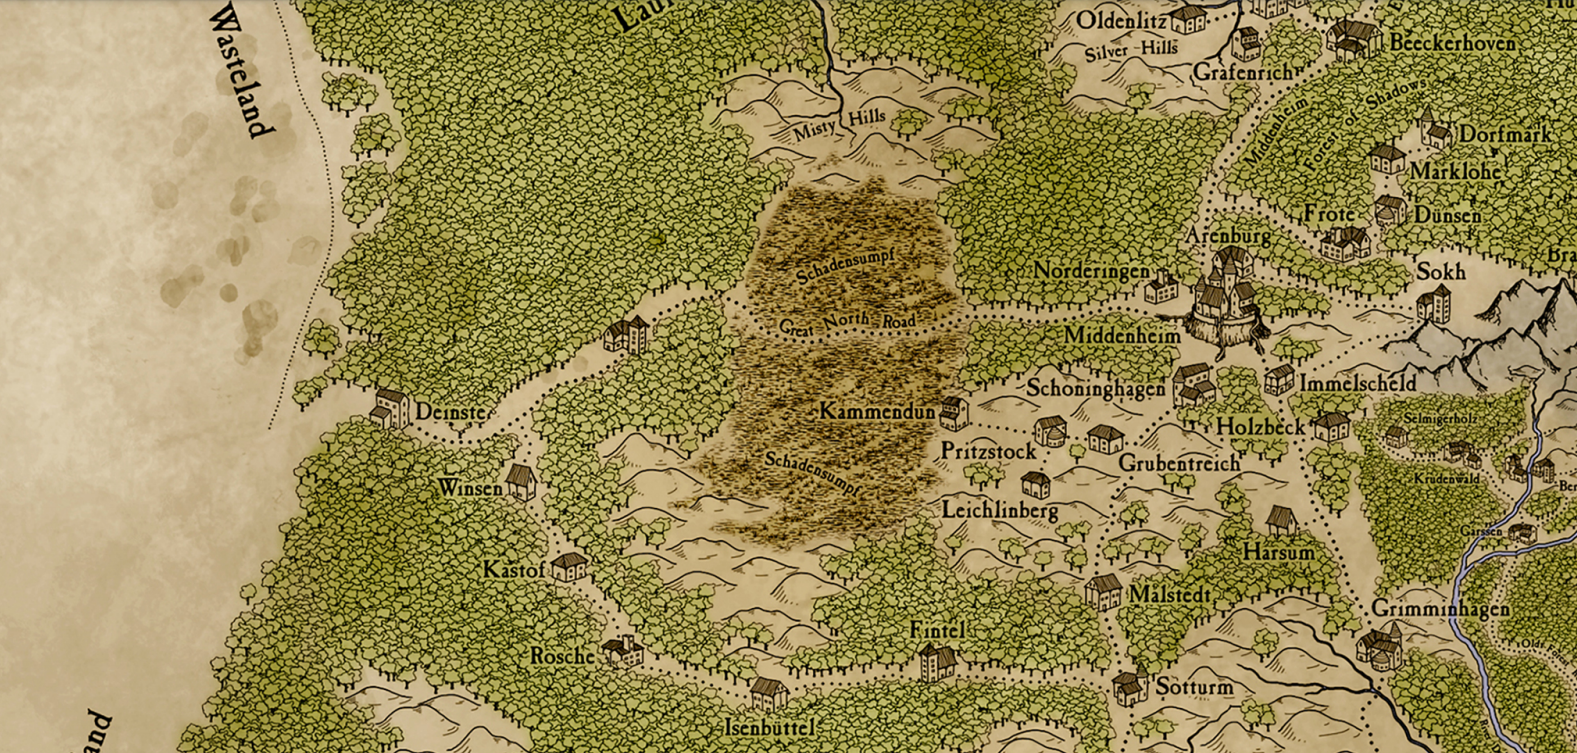
\includegraphics[width=\textwidth]{carte locale.png}
\end{document}